
\usepackage[utf8]{inputenc}
\usepackage[english]{babel}
\usepackage{amsmath}
\usepackage{amssymb}
\usepackage{amsthm}
\usepackage{yhmath}
\usepackage{gensymb}
\usepackage{graphicx}
\usepackage{siunitx}
\usepackage{amscd}
\usepackage{sectsty}
\usepackage{stmaryrd}
\usepackage{tikz-cd}
\usepackage{wrapfig}
\usepackage{xcolor}
\usepackage[margin=1.5in]{geometry}
\usepackage[framemethod=TikZ]{mdframed}
\usepackage{eso-pic}
\usepackage{import}

\theoremstyle{definition}
\newtheorem{thm}{Teorema}[subsection]
%\newtheorem*{exm}{Esempio}
\renewcommand\qedsymbol{$\blacksquare$}
\addto\captionsenglish{\renewcommand*{\proofname}{Dimostrazione}}
\addto\captionsenglish{\renewcommand{\contentsname}{Indice}}

\sectionfont{\fontsize{20}{15}\selectfont}
\subsectionfont{\fontsize{14}{15}\selectfont}

\renewcommand\thefootnote{\textcolor{red}{\arabic{footnote}}}

%%
\usepackage{xcolor}
\newtheoremstyle{example}
  {}
  {}
  {\itshape}
  {}
  {\bfseries}
  {}
  { }
  {\colorbox{red!20}{#1.}}

\theoremstyle{example}
\newtheorem*{exm}{Esempio}
%%
%%
\newtheoremstyle{observation}
  {}
  {}
  {\itshape}
  {}
  {\bfseries}
  {}
  { }
  {\colorbox{blue!20}{#1.}}

\theoremstyle{observation}
\newtheorem*{obs}{Osservazione}
%%

\newcommand{\id}{\operatorname{id}}
\newcommand{\Mat}{\operatorname{Mat}}
\newcommand{\supp}{\operatorname{supp}}
\newcommand{\quot}{\operatorname{quot}}
\newcommand{\tor}{\operatorname{tor}}
\newcommand{\sat}{\operatorname{sat}}
\newcommand{\Ann}{\operatorname{Ann}}
\newcommand{\spec}{\operatorname{spec}}
\newcommand{\con}{\operatorname{con}}
\newcommand{\valpha}{\underline{\alpha}}
\newcommand{\vbeta}{\underline{\beta}}
\newcommand{\vgamma}{\underline{\gamma}}
\newcommand{\vdelta}{\underline{\delta}}
\newcommand{\vepsilon}{\underline{\varepsilon}}
\newcommand{\rbar}{r\underline{\, \, \,}}
\newcommand{\sbar}{s\underline{\, \, \,}}
\newcommand{\tbar}{t\underline{\, \, \,}}

\newcommand\BackgroundPic{%
\put(0,0){%
\parbox[b][\paperheight]{\paperwidth}{%
\vfill
\centering
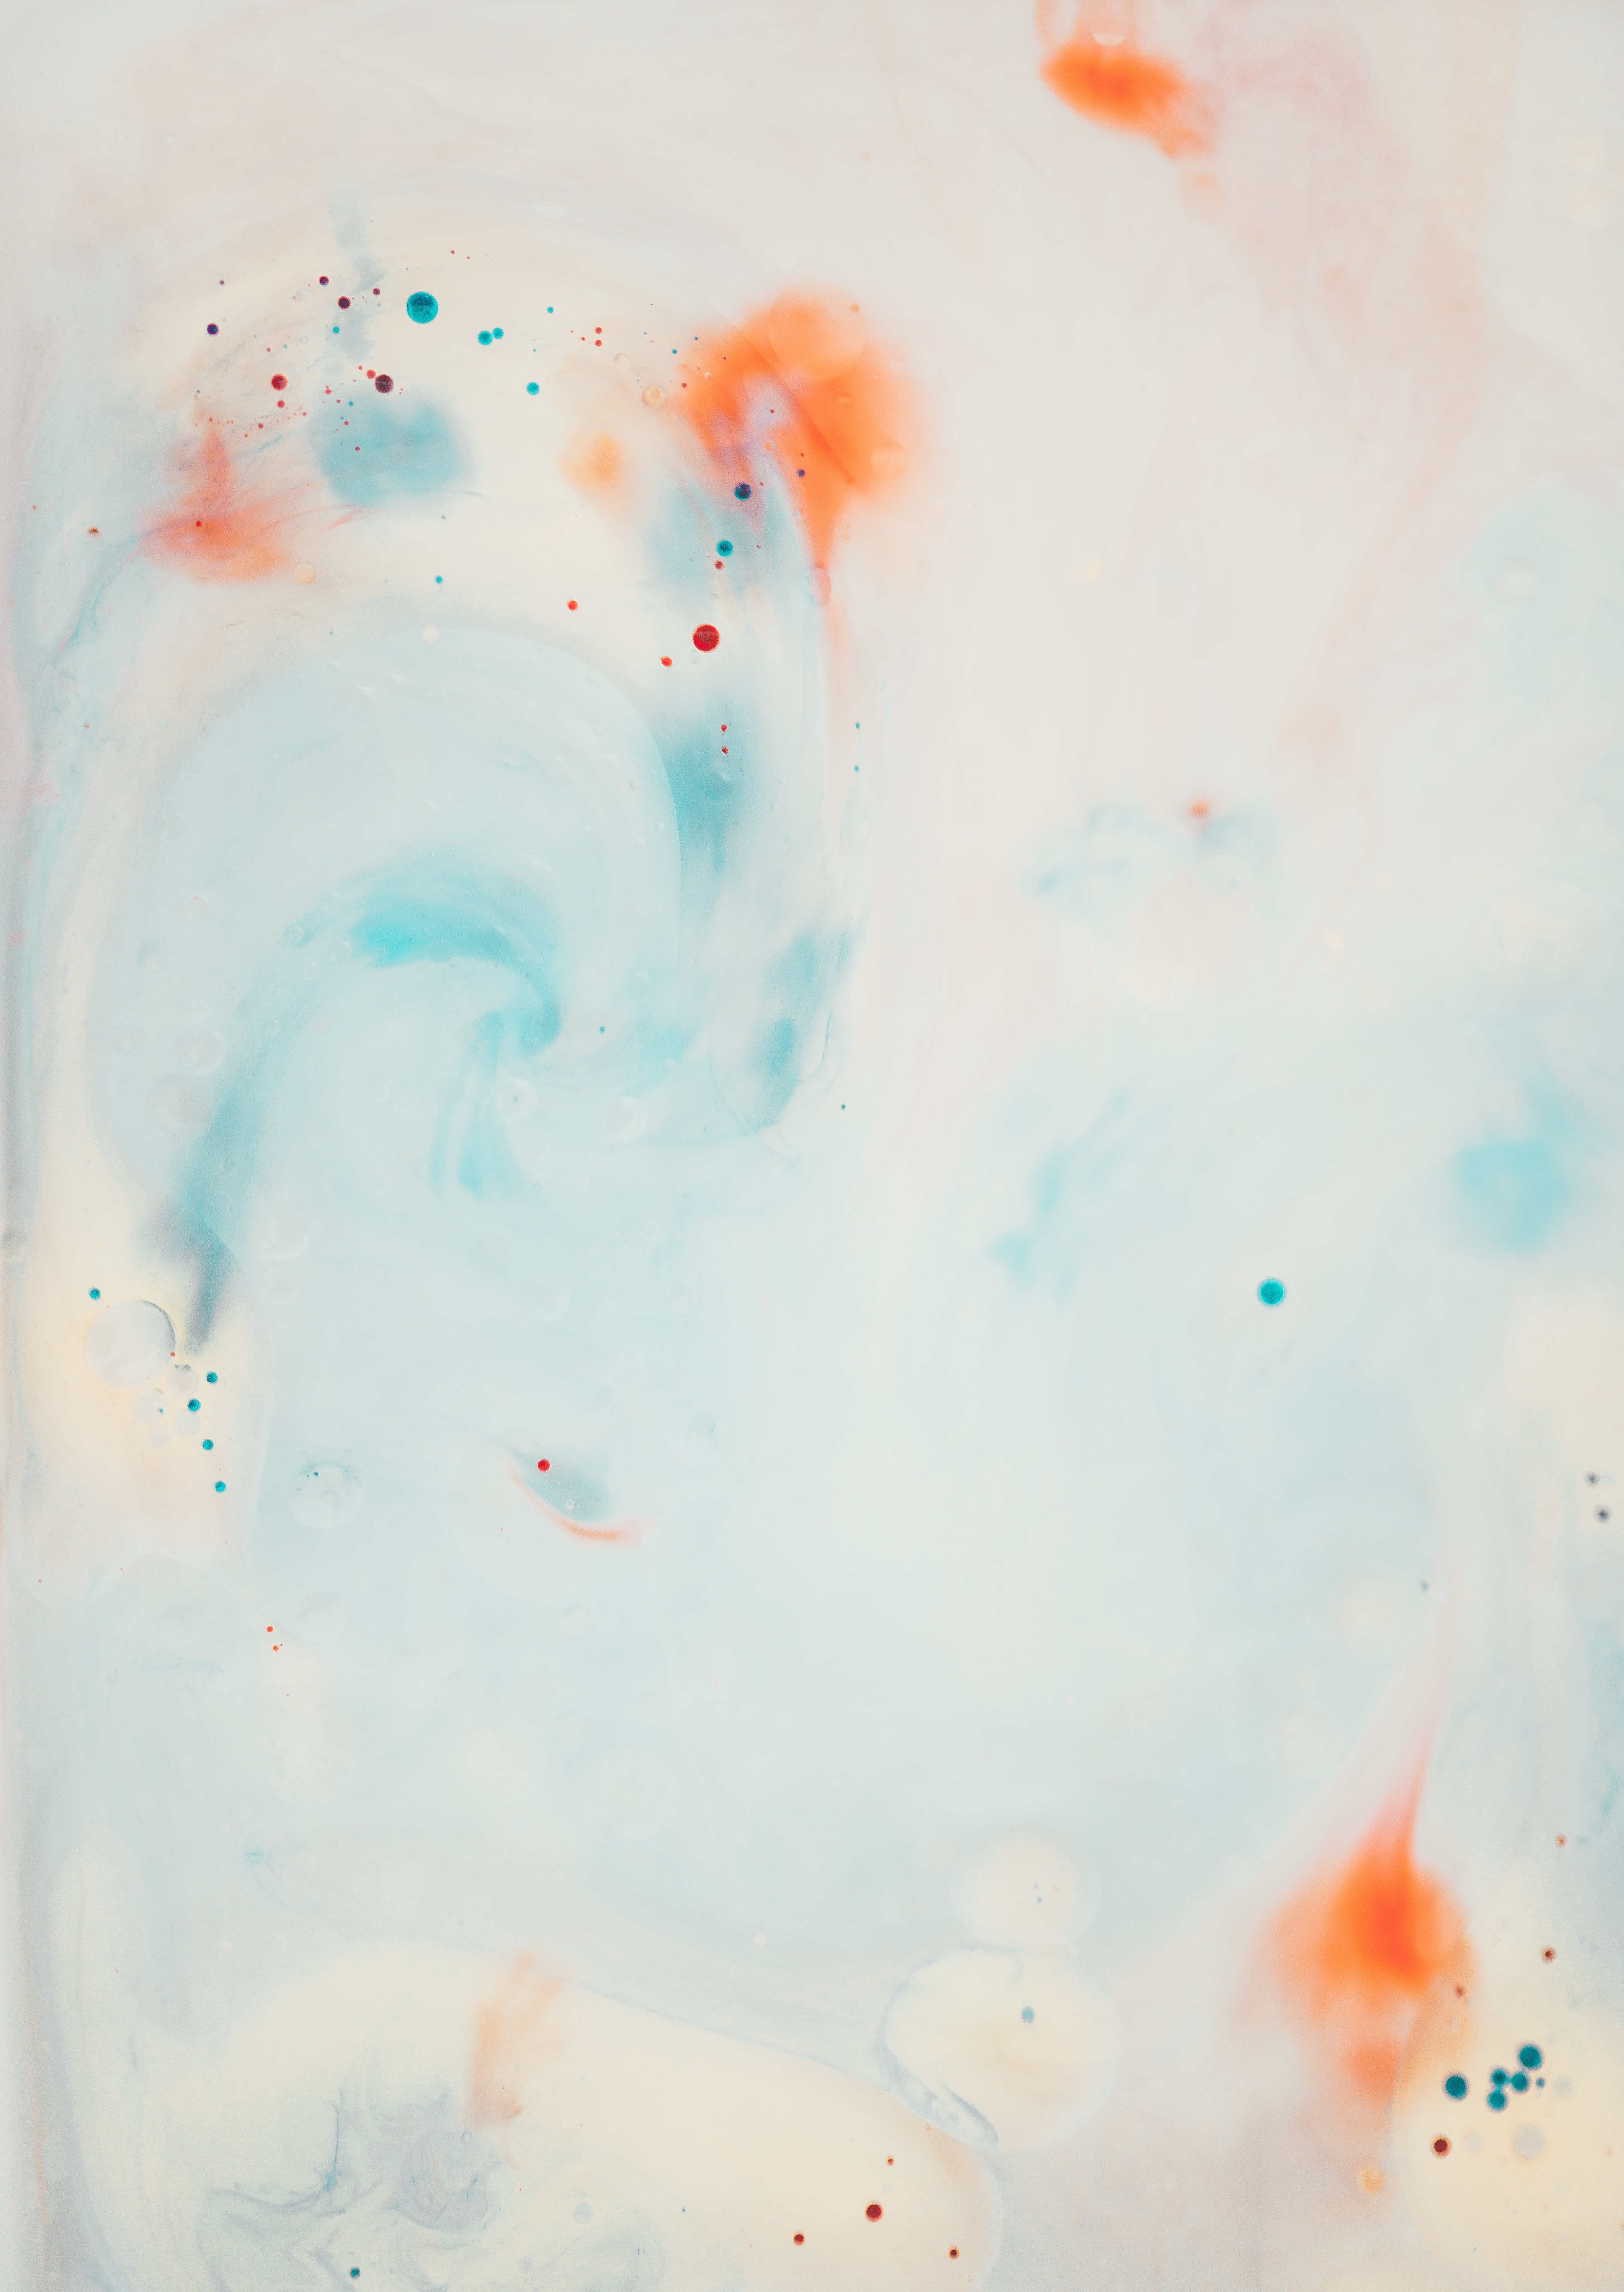
\includegraphics[width=\paperwidth,height=\paperheight]{Fractal.png}%
\vfill
}}}

%shortcut to mathbb
\newcommand{\N}{\mathbb{N}}
\newcommand{\Z}{\mathbb{Z}}
\newcommand{\Q}{\mathbb{Q}}
\newcommand{\R}{\mathbb{R}}
\newcommand{\I}{\mathbb{I}}
\newcommand{\C}{\mathbb{C}}

%%%%%%%%%%%%%%%%%%%%%%%%%%%%%%
% Ricordati di mettere sempre le label
%%%%%%%%%%%%%%%%%%%%%%%%%%%%%%
%Theorem
\newcounter{teo}[subsection] \setcounter{teo}{0}
\renewcommand{\theteo}{\arabic{section}.\arabic{subsection}.\arabic{teo}}
\newenvironment{teo}[2][]{%
  \refstepcounter{teo}%
  \ifstrempty{#1}%
  % if condition (without title)
  {\mdfsetup{%
      frametitle={%
          \tikz[baseline=(current bounding box.east),outer sep=0pt]
          \node[anchor=east,rectangle,fill=cyan!20]
          {\strut Teorema~\theteo};}
      }%
  % else condition (with title)
  }{\mdfsetup{%
      frametitle={%
          \tikz[baseline=(current bounding box.east),outer sep=0pt]
          \node[anchor=east,rectangle,fill=cyan!20]
          {\strut Teorema~\theteo:~#1};}%
      }%
  }%
  % Both conditions
  \mdfsetup{%
      innertopmargin=5pt,linecolor=cyan!20,%
      linewidth=2pt,topline=true,%
      frametitleaboveskip=\dimexpr-\ht\strutbox\relax%
  }
\begin{mdframed}[]\relax%
\label{#2}}{\end{mdframed}}
%%%%%%%%%%%%%%%%%%%%%%%%%%%%%%

%%%%%%%%%%%%%%%%%%%%%%%%%%%%%%
% Lemma
\newenvironment{lem}[2][]{%
  \refstepcounter{teo}%
  \ifstrempty{#1}%
  % if condition (without title)
  {\mdfsetup{%
      frametitle={%
          \tikz[baseline=(current bounding box.east),outer sep=0pt]
          \node[anchor=east,rectangle,fill=cyan!20]
          {\strut Lemma~\theteo};}
      }%
  % else condition (with title)
  }{\mdfsetup{%
      frametitle={%
          \tikz[baseline=(current bounding box.east),outer sep=0pt]
          \node[anchor=east,rectangle,fill=cyan!20]
          {\strut Lemma~\theteo:~#1};}%
      }%
  }%
  % Both conditions
  \mdfsetup{%
      innertopmargin=5pt,linecolor=cyan!20,%
      linewidth=2pt,topline=true,%
      frametitleaboveskip=\dimexpr-\ht\strutbox\relax%
  }
\begin{mdframed}[]\relax%
\label{#2}}{\end{mdframed}}
%%%%%%%%%%%%%%%%%%%%%%%%%%%%%%

%%%%%%%%%%%%%%%%%%%%%%%%%%%%%%
% Proposizione
\newenvironment{prop}[2][]{%
  \refstepcounter{teo}%
  \ifstrempty{#1}%
  % if condition (without title)
  {\mdfsetup{%
      frametitle={%
          \tikz[baseline=(current bounding box.east),outer sep=0pt]
          \node[anchor=east,rectangle,fill=cyan!20]
          {\strut Proposizione~\theteo};}
      }%
  % else condition (with title)
  }{\mdfsetup{%
      frametitle={%
          \tikz[baseline=(current bounding box.east),outer sep=0pt]
          \node[anchor=east,rectangle,fill=cyan!20]
          {\strut Proposizione~\theteo:~#1};}%
      }%
  }%
  % Both conditions
  \mdfsetup{%
      innertopmargin=5pt,linecolor=cyan!20,%
      linewidth=2pt,topline=true,%
      frametitleaboveskip=\dimexpr-\ht\strutbox\relax%
  }
\begin{mdframed}[]\relax%
\label{#2}}{\end{mdframed}}
%%%%%%%%%%%%%%%%%%%%%%%%%%%%%%

%%%%%%%%%%%%%%%%%%%%%%%%%%%%%%
% Corollario
\newenvironment{cor}[2][]{%
  \refstepcounter{teo}%
  \ifstrempty{#1}%
  % if condition (without title)
  {\mdfsetup{%
      frametitle={%
          \tikz[baseline=(current bounding box.east),outer sep=0pt]
          \node[anchor=east,rectangle,fill=cyan!20]
          {\strut Corollario~\theteo};}
      }%
  % else condition (with title)
  }{\mdfsetup{%
      frametitle={%
          \tikz[baseline=(current bounding box.east),outer sep=0pt]
          \node[anchor=east,rectangle,fill=cyan!20]
          {\strut Corollario~\theteo:~#1};}%
      }%
  }%
  % Both conditions
  \mdfsetup{%
      innertopmargin=5pt,linecolor=cyan!20,%
      linewidth=2pt,topline=true,%
      frametitleaboveskip=\dimexpr-\ht\strutbox\relax%
  }
\begin{mdframed}[]\relax%
\label{#2}}{\end{mdframed}}
%%%%%%%%%%%%%%%%%%%%%%%%%%%%%%

%%%%%%%%%%%%%%%%%%%%%%%%%%%%%%
% Definition
\newenvironment{defn}[2][]{%
  \refstepcounter{teo}%
  \ifstrempty{#1}%
  % if condition (without title)
  {\mdfsetup{%
      frametitle={%
          \tikz[baseline=(current bounding box.east),outer sep=0pt]
          \node[anchor=east,rectangle,fill=yellow!40]
          {\strut Definizione~\theteo};}
      }%
  % else condition (with title)
  }{\mdfsetup{%
      frametitle={%
          \tikz[baseline=(current bounding box.east),outer sep=0pt]
          \node[anchor=east,rectangle,fill=yellow!40]
          {\strut Definizione~\theteo:~#1};}%
      }%
  }%
  % Both conditions
  \mdfsetup{%
      innertopmargin=5pt,linecolor=yellow!40,%
      linewidth=2pt,topline=true,%
      frametitleaboveskip=\dimexpr-\ht\strutbox\relax%
  }
\begin{mdframed}[]\relax%
\label{#2}}{\end{mdframed}}
%%%%%%%%%%%%%%%%%%%%%%%%%%%%%%

%%%%%%%%%%%%%%%%%%%%%%%%%%%%%%
% Observation
\newenvironment{observ}[2][]{%
  \refstepcounter{teo}%
  \ifstrempty{#1}%
  % if condition (without title)
  {\mdfsetup{%
      frametitle={%
          \tikz[baseline=(current bounding box.east),outer sep=0pt]
          \node[anchor=east,rectangle,fill=blue!20]
          {\strut Osservazione~\theteo};}
      }%
  % else condition (with title)
  }{\mdfsetup{%
      frametitle={%
          \tikz[baseline=(current bounding box.east),outer sep=0pt]
          \node[anchor=east,rectangle,fill=blue!20]
          {\strut Osservazione~\theteo:~#1};}%
      }%
  }%
  % Both conditions
  \mdfsetup{%
      innertopmargin=5pt,linecolor=blue!20,%
      linewidth=2pt,topline=true,%
      frametitleaboveskip=\dimexpr-\ht\strutbox\relax%
  }
\begin{mdframed}[]\relax%
\label{#2}}{\end{mdframed}}
%%%%%%%%%%%%%%%%%%%%%%%%%%%%%%

%%%%%%%%%%%%%%%%%%%%%%%%%%%%%%
% Example
\newenvironment{example}[2][]{%
  \refstepcounter{teo}%
  \ifstrempty{#1}%
  % if condition (without title)
  {\mdfsetup{%
      frametitle={%
          \tikz[baseline=(current bounding box.east),outer sep=0pt]
          \node[anchor=east,rectangle,fill=red!20]
          {\strut Esempio~\theteo};}
      }%
  % else condition (with title)
  }{\mdfsetup{%
      frametitle={%
          \tikz[baseline=(current bounding box.east),outer sep=0pt]
          \node[anchor=east,rectangle,fill=red!20]
          {\strut Esempio~\theteo:~#1};}%
      }%
  }%
  % Both conditions
  \mdfsetup{%
      innertopmargin=5pt,linecolor=red!20,%
      linewidth=2pt,topline=true,%
      frametitleaboveskip=\dimexpr-\ht\strutbox\relax%
  }
\begin{mdframed}[]\relax%
\label{#2}}{\end{mdframed}}
%%%%%%%%%%%%%%%%%%%%%%%%%%%%%%